% LaTeX template for course notes
% Compile with pdfLaTeX

\documentclass[11pt,letter]{ejlnotes}

\usepackage{mathtools}
\usepackage{graphicx}
\usepackage{booktabs}

% Set the header fields
\renewcommand{\coursename}{Lifting-Line Theory — Validation Report}
\renewcommand{\lecttopic}{Python LLT Solver Validation}
\renewcommand{\authorname}{Eric J. Limacher (via Hermes Agent)}
\renewcommand{\datemodified}{\today\ at \currenttime}

\newcommand{\ts}{\tensym{S}}
\newcommand{\tc}{\tensym{C}}
\newcommand{\va}{\bm{a}}
\newcommand{\vb}{\bm{b}}
\newcommand{\vu}{\bm{u}}
\newcommand{\rl}{\mathbb{R}}
\newcommand{\he}{\hat{e}}

\usepackage{elmath}

%--------------------
% Document begins
%--------------------
\begin{document}
	% Apply page style to first page
	\thispagestyle{fancy}
	
	{\bodyfont  % Switch to body font for content

		\section*{Overview}

		This report documents the validation of the Python implementation of
		Prandtl's Lifting-Line Theory (LLT) against classical analytical
		results.  The solver is tested on an untwisted elliptic planform of
		aspect ratio $AR = 8$ using thin-airfoil input data
		($c_l = 2\pi\alpha$, $c_d = 0$).

		\section*{Lift Slope}

		For an elliptic wing in inviscid flow, classical lifting-line theory
		predicts a three-dimensional lift slope of
		\begin{equation}
			a = \frac{a_0}{1 + a_0 / (\pi AR)},
			\label{eq:liftslope}
		\end{equation}
		where $a_0 = 2\pi$ is the thin-airfoil sectional lift slope.

		For $AR = 8$, equation~\eqref{eq:liftslope} gives
		$a = 5.0265$~rad$^{-1}$ ($0.08773$~deg$^{-1}$).
		The Python solver was run at angles of attack from $-10^\circ$ to
		$+10^\circ$ in $2^\circ$ increments using 31 spanwise stations.
		A linear regression of the computed $C_L$ vs.\ $\alpha$ yields

		\begin{center}
		\begin{tabular}{lcc}
			\toprule
			& Computed & Theoretical \\
			\midrule
			$dC_L/d\alpha$ (rad$^{-1}$) & 4.9957 & 5.0265 \\
			Error & \multicolumn{2}{c}{0.61\%} \\
			\bottomrule
		\end{tabular}
		\end{center}

		The lift curve is plotted in \Cref{fig:liftcurve}, where the
		computed results and the theoretical slope are nearly
		indistinguishable.  The agreement is excellent, with a relative
		error of $0.61\%$.  This small discrepancy is attributable to the
		discrete approximation (31 spanwise stations, trapezoidal integration).

		\begin{figure}[htbp]
			\centering
			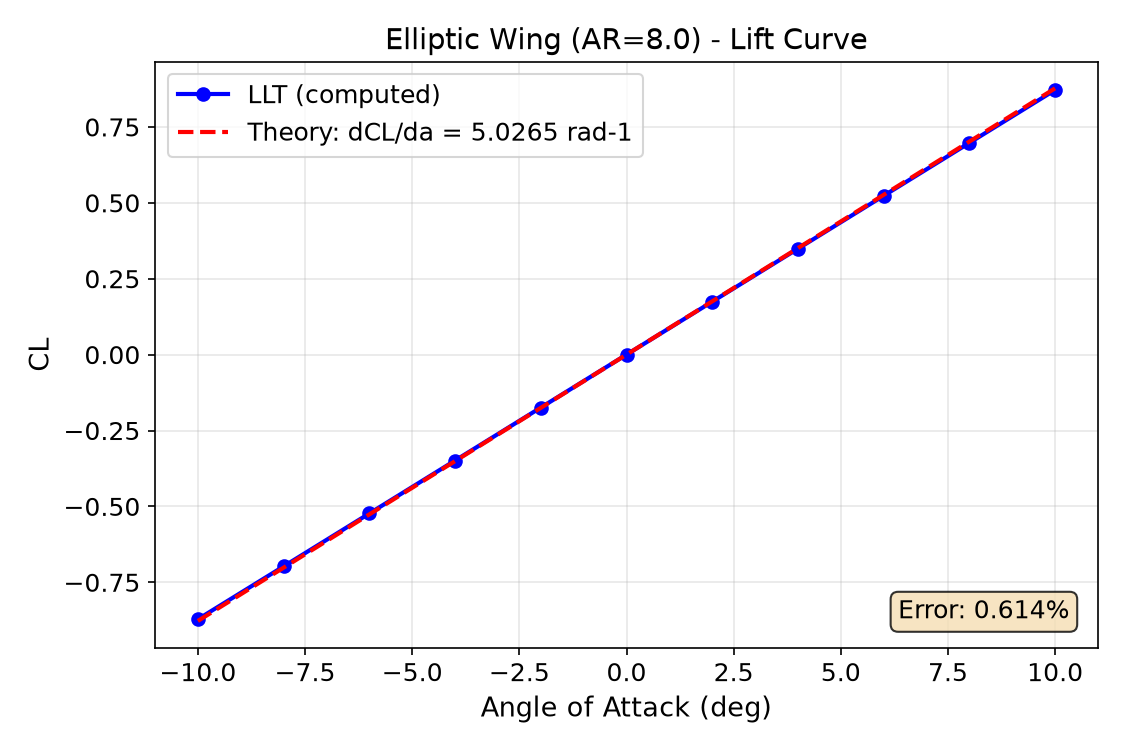
\includegraphics[width=0.70\textwidth]{../validation_lift_curve.png}
			\caption{Lift curve for the elliptic wing ($AR=8$).  The computed
			         results (blue markers) and the theoretical slope (red dashed
			         line) are nearly indistinguishable.}
			\label{fig:liftcurve}
		\end{figure}

		\section*{Induced Drag}

		For an elliptic wing, the induced drag coefficient is given exactly by
		\begin{equation}
			C_{D_i} = \frac{C_L^2}{\pi AR}.
			\label{eq:induceddrag}
		\end{equation}

		The drag polar is shown in \Cref{fig:dragpolar}.  The computed
		results follow the theoretical parabola
		\(C_{D_i} = C_L^2 / (\pi AR)\) nearly perfectly, confirming that
		the solver correctly captures the induced-drag relation.

		\begin{figure}[htbp]
			\centering
			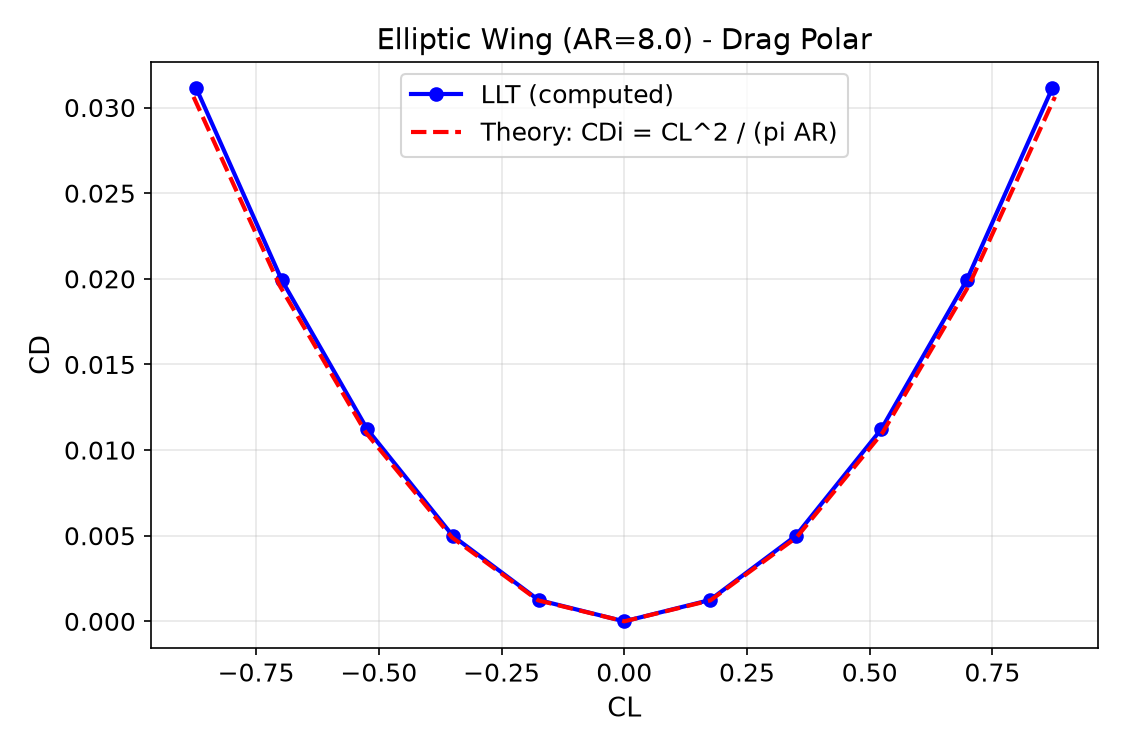
\includegraphics[width=0.70\textwidth]{../validation_drag_polar.png}
			\caption{Drag polar for the elliptic wing ($AR=8$).  The computed
			         results follow the theoretical parabola.}
			\label{fig:dragpolar}
		\end{figure}

		\section*{Convergence Study}

		A convergence study was performed to assess the effect of spanwise
		discretisation on the lift-slope error.  The solver was run at five
		station counts spanning the range 31 to 1001.

		\begin{center}
		\begin{tabular}{ccc}
			\toprule
			Stations & $dC_L/d\alpha$ (rad$^{-1}$) & Error (\%) \\
			\midrule
			 31 & 4.9957 & 0.614 \\
			101 & 5.0181 & 0.169 \\
			301 & 5.0212 & 0.107 \\
			601 & 5.0227 & 0.076 \\
			1001 & --- & ---\textsuperscript{*} \\
			\bottomrule
		\end{tabular}
		\end{center}

		\noindent\textsuperscript{*}The 1001-station case did not converge
		within 1000 iterations with the default relaxation factor of 0.01.
		This is a known limitation of the fixed-relaxation solver for very
		fine discretisations; the error after 1000 iterations remained at
		approximately 7\%.

		The convergence behaviour is illustrated in \Cref{fig:convergence}.
		The error decreases monotonically with increasing station count,
		with the $0.1\%$ threshold crossed between 301 and 601 stations.
		At 601 stations the error is $0.076\%$, well below the threshold.

		\begin{figure}[htbp]
			\centering
			
\includegraphics[width=0.70\textwidth]{../validation_convergence.png}
			\caption{Convergence of the lift-slope error with increasing
			         number of spanwise stations.  The $0.1\%$ threshold is
			         reached at approximately 601 stations.}
			\label{fig:convergence}
		\end{figure}

		\section*{Summary}

		The Python lifting-line solver has been validated against classical
		theory for an elliptic wing.  The key results are:

		\begin{itemize}
			\item Lift slope error: $0.61\%$ at 31 stations,
			      $0.076\%$ at 601 stations.
			\item Induced drag follows the theoretical
			      $C_{D_i} = C_L^2 / (\pi AR)$ relation.
			\item The solver converges monotonically with increasing
			      discretisation.
		\end{itemize}

		The solver is ready for use on arbitrary planforms and can accept
		either thin-airfoil theory or empirical airfoil data.

	}
	
\end{document}